\section{Background Modelling}
\label{sec:background_model}



\subsection{Background modeling strategy}
\label{ssec:bkg_strategy}

The strategy for the continuous background modelling follows what traditionally done in $H\to\gamma\gamma$ measurements, with the addition of some dedicated procedures to cope with specific issues related to insufficient MC statistics or very low-statistics categories. This section only contains a simplified description, more details could be found in HGam coupling analysis ~\ref{ANA-HIGG-2020-16-INT1}. 

The steps comprising the background modelling strategy can be summarised as follows:
\begin{itemize}

  \item The composition of the continuous background in term of \yy, \yjet and \jetjet components is estimated with data driven technique for each category entering the measurement, as detailed in \Sect{\ref{ssec:bkg_composition}}.
  \item The background fractions are used to build \myy background templates for each category entering the measurement, where the \yy component is obtained from MC, while the \yjet and \jetjet components are measured from data driven control regions and used to reweight the \yy MC, as detailed in \Sect{\ref{ssec:bkg_templates}}.

  \item In order to improve the background modeling and reduce the impact of limited MC statistics, a smoothing procedure is being developed to be eventually applied to the background template, provided that the improvements on the results outweight the possible associated systematic uncertainties. 

  \item The Spurious Signal approach is used in the smoothed \yy templates to select a functional form to describe each template, as well as the associated bias that will enter the measurement as a systematic uncertainties, as detailed in \Sect{\ref{ssec:spurious_signal}}. The Spurious Signal criteria are defined in order to cope with the limited MC statistics that in some case leads to non-physical large bias measurements.

  \item In very low-statistic categories, defined as those categories with \textcolor{red}{less than 10 events per bin in the \myy sidebands}, the smoothing procedure tends to introduce large non-physical structures in the templates, and it is therefore not suited to be used for them. For this reason, for this categories we initially select the statistically-justified function performing a Wald-test on the data sidebands using a family of function based on a exponential of increasing complexity. We accept the simplest function justifies by the Wald-test, and perform the Spurious Signal measurement with this function tolerating a bias that could be larger than the criteria used for the high-statistic categories, but would have a small impact on the overall sensitivity. This procedure is described in \Sect{\ref{sssec:bkg_functions}}. 

\end{itemize}


\subsection{Background compositions}
\label{ssec:bkg_composition}

The dominant background entering the invariant mass spectrum comes from SM continuum diphoton production. A large number of photons are produced inside jets due to de decays of neutral mesons to photon pairs. Thus, photon-jet and di-jet events in which the jets are mis-identified as photons represent a non-negligible source of background. Photon-pairs can be also faked from Drell-Yan events in which both electrons are misidentified as photons. However, this background only contributes with a small fraction ($<1\%$).

The number of \yy, \yjet and \jetjet events entering each category after the final selection is estimated by means of a double two-dimensional sideband ABCD method~\cite{ATL-COM-PHYS-2012-592}. This data-driven method extrapolates the fraction of fake photons within the signal region from the composition of the side-band control regions, built by inverting photon identification and isolation requirements. The fractions are calculated individually in each categories and OO bins for the background template building. Table ~\ref{tab:yyfraction} lists the \yy fraction in all categories. More details are shown in Appendix ~\ref{appendix:2x2DSB}. 

\begin{table}[htbp]
  \centering
  \begin{tabular}{c|cccc}
  \toprule
           &  TT  &  TL  &  LT  &  LL  \\ 
  \toprule
  OO bin1  & $0.76 \pm 0.16$ & $0.90 \pm 0.10$ & $0.93 \pm 0.03$ & $0.86 \pm 0.05$ \\ \hline
  OO bin2  & $0.89 \pm 0.10$ & $0.81 \pm 0.10$ & $0.81 \pm 0.06$ & $0.87 \pm 0.07$ \\ \hline
  OO bin3  & $0.79 \pm 0.15$ & $0.75 \pm 0.12$ & $0.88 \pm 0.03$ & $0.83 \pm 0.06$ \\ \hline
  OO bin4  & $0.92 \pm 0.08$ & $0.81 \pm 0.09$ & $0.84 \pm 0.05$ & $0.90 \pm 0.05$ \\ \hline
  OO bin5  & $0.78 \pm 0.14$ & $0.81 \pm 0.10$ & $0.86 \pm 0.05$ & $0.88 \pm 0.07$ \\ \hline
  OO bin6  & $0.88 \pm 0.10$ & $0.87 \pm 0.09$ & $0.88 \pm 0.05$ & $0.83 \pm 0.04$ \\
  \bottomrule
  \end{tabular}
  \caption{\yy fraction calculated with double two-dimensional sideband ABCD method. \yjet and \jetjet components are merged together in following analysis, so the fraction is $1-f_{\yy}$. }
  \label{tab:yyfraction}
\end{table}

\begin{figure}[tbp]
  \centering
  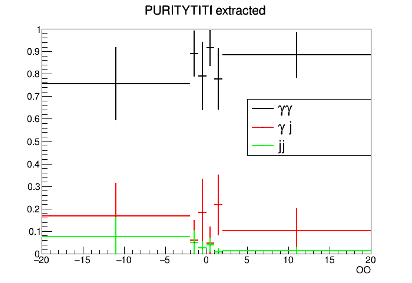
\includegraphics[width=0.45\linewidth]{figure/bkgtmpls/TT/yyfrac_TT.png}
  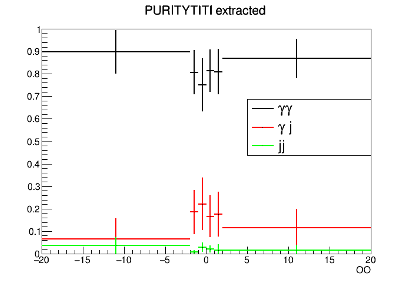
\includegraphics[width=0.45\linewidth]{figure/bkgtmpls/TL/yyfrac_TL.png} \\
  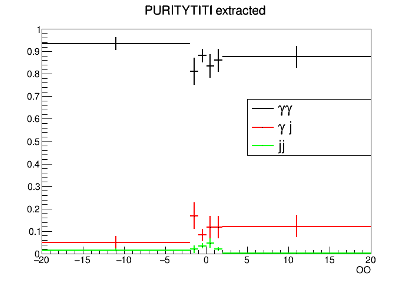
\includegraphics[width=0.45\linewidth]{figure/bkgtmpls/LT/yyfrac_LT.png}
  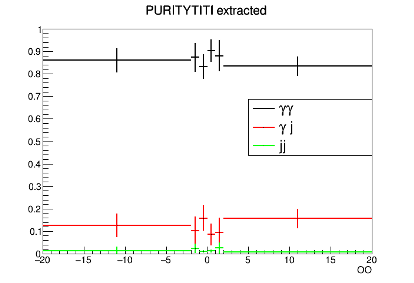
\includegraphics[width=0.45\linewidth]{figure/bkgtmpls/LL/yyfrac_LL.png} 
  \caption{\yy, \yjet, \jetjet fraction in TT(upper left), TL(upper right), LT(bottom left), LL(bottom right) categories, as a function of OO. }
  \label{fig:yyfraction}
\end{figure}



\clearpage
\subsection{Background templates}
\label{ssec:bkg_templates}

Considering the low \jetjet fraction and similar performance of \yjet and \jetjet, those two components are merged together as \yjet+\jetjet for the background estimation. The shape is determined with a data control region, in TT, TL and LT categories it is defined as at least one of the two selected photons fail the tight identification and loose isolation requirement due to insufficient MC statistics, and in LL category it is defined as inverting the identification and isolation of exactly one of two photon candidates.
Contamination from \yy has been tested to be ignorable as shown in Figure ~\ref{fig:yjCR}, and a \textcolor{red}{linear} reweighting is derived to match the \yy and control region shapes. The bin width for ratio function smoothing varies from 5GeV, 2GeV, 1GeV and 0.5GeV respectively in TT, TL, LT, LL categories to match the MC statistics for an un-biased result. Uncertainty of this reweighted template contains two part: from the choice of smoothing function and from \yy fraction, while the latter is dominant. 
These derived shapes are combined with the measured relative event fractions to obtain the total background shape. The \yy fraction is measured as mentioned in ~\ref{ssec:bkg_composition} \\

The obtained templates show a good agreement when comparing them with events in data passing the nominal selection (with tight photon identification and isolation cuts, TI) in the sidebands, as shown in \Fig{\ref{fig:BkgData-MC}}.\\

\clearpage
\begin{figure}[htbp]
  \centering
  \subfloat[TT category OO bin1]{ 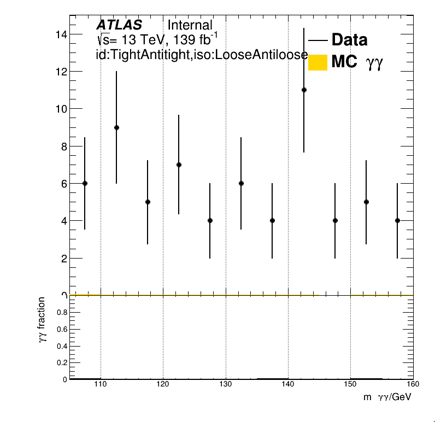
\includegraphics[width= 0.30\textwidth]{figure/bkgtmpls/TT/CR/b1.png} }
  \subfloat[TT category OO bin2]{ 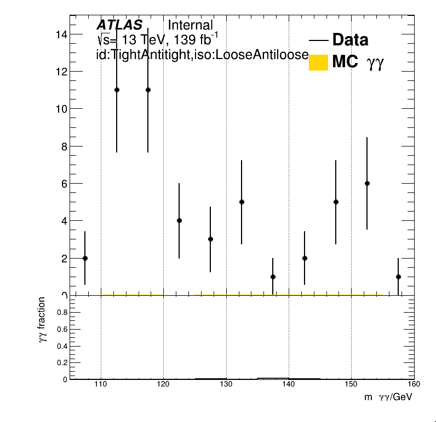
\includegraphics[width= 0.30\textwidth]{figure/bkgtmpls/TT/CR/b2.png} }
  \subfloat[TT category OO bin3]{ 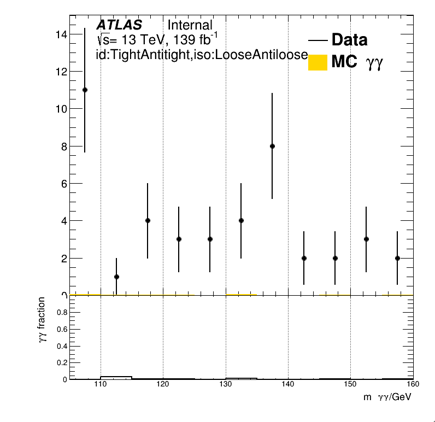
\includegraphics[width= 0.30\textwidth]{figure/bkgtmpls/TT/CR/b3.png} } \\
  \subfloat[TT category OO bin4]{ 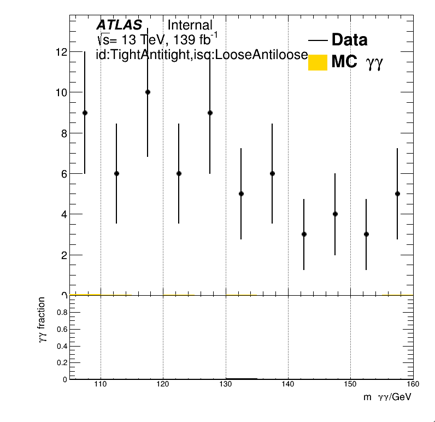
\includegraphics[width= 0.30\textwidth]{figure/bkgtmpls/TT/CR/b4.png} }
  \subfloat[TT category OO bin5]{ 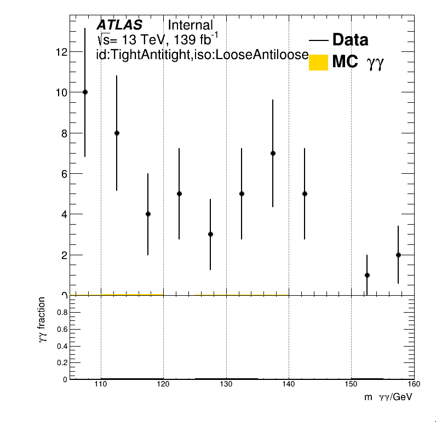
\includegraphics[width= 0.30\textwidth]{figure/bkgtmpls/TT/CR/b5.png} }
  \subfloat[TT category OO bin6]{ 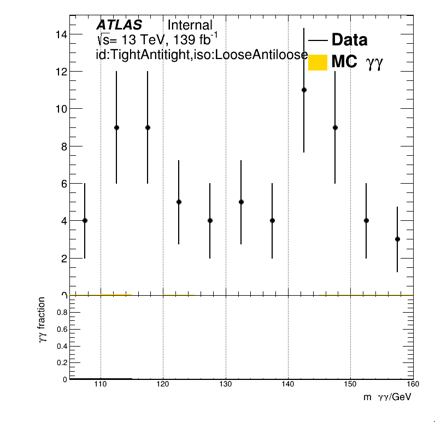
\includegraphics[width= 0.30\textwidth]{figure/bkgtmpls/TT/CR/b6.png} } \\
  \subfloat[TL category OO bin1]{ 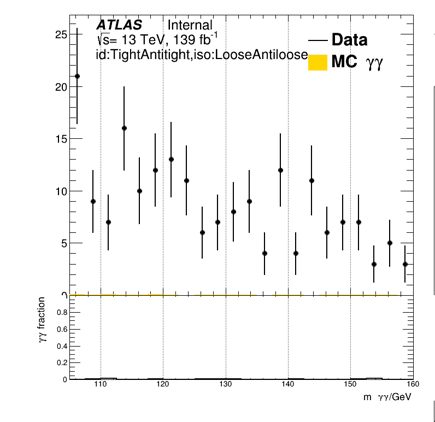
\includegraphics[width= 0.30\textwidth]{figure/bkgtmpls/TL/CR/b1.png} }
  \subfloat[TL category OO bin2]{ 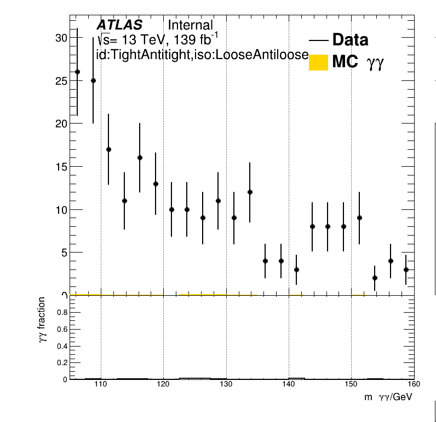
\includegraphics[width= 0.30\textwidth]{figure/bkgtmpls/TL/CR/b2.png} }
  \subfloat[TL category OO bin3]{ 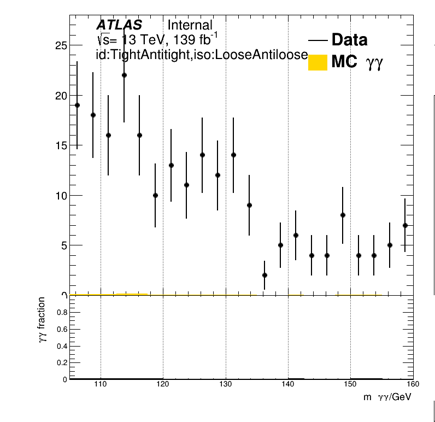
\includegraphics[width= 0.30\textwidth]{figure/bkgtmpls/TL/CR/b3.png} } \\
  \subfloat[TL category OO bin4]{ 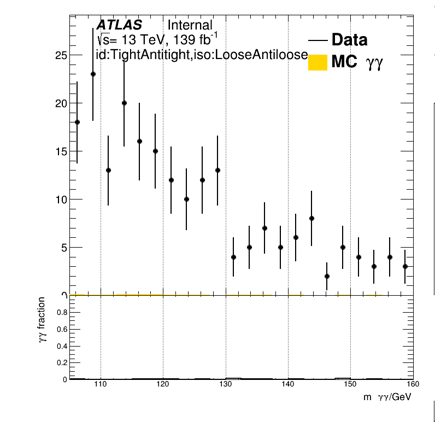
\includegraphics[width= 0.30\textwidth]{figure/bkgtmpls/TL/CR/b4.png} }
  \subfloat[TL category OO bin5]{ 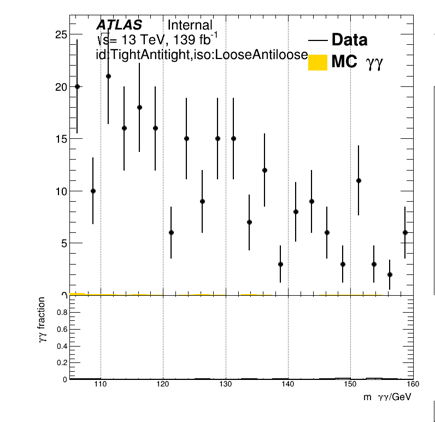
\includegraphics[width= 0.30\textwidth]{figure/bkgtmpls/TL/CR/b5.png} }
  \subfloat[TL category OO bin6]{ 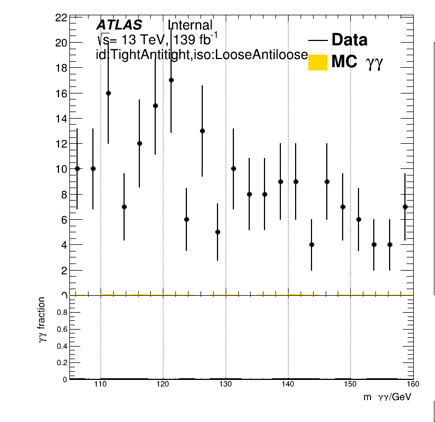
\includegraphics[width= 0.30\textwidth]{figure/bkgtmpls/TL/CR/b6.png} } \\
\end{figure}
\clearpage
\begin{figure}[htbp]
\centering
  \subfloat[LT category OO bin1]{ 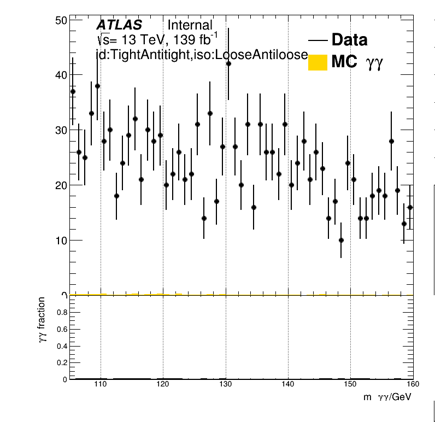
\includegraphics[width= 0.30\textwidth]{figure/bkgtmpls/LT/CR/b1.png} }
  \subfloat[LT category OO bin2]{ 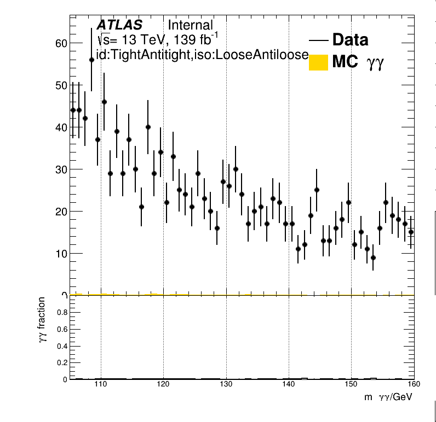
\includegraphics[width= 0.30\textwidth]{figure/bkgtmpls/LT/CR/b2.png} }
  \subfloat[LT category OO bin3]{ 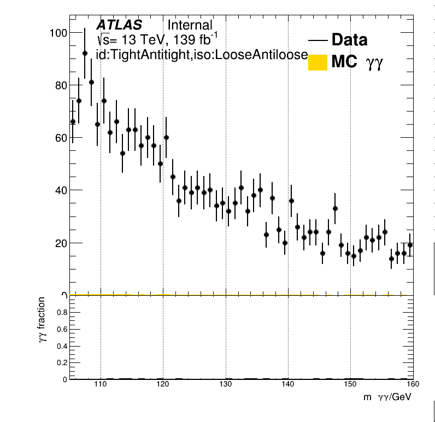
\includegraphics[width= 0.30\textwidth]{figure/bkgtmpls/LT/CR/b3.png} } \\
  \subfloat[LT category OO bin4]{ 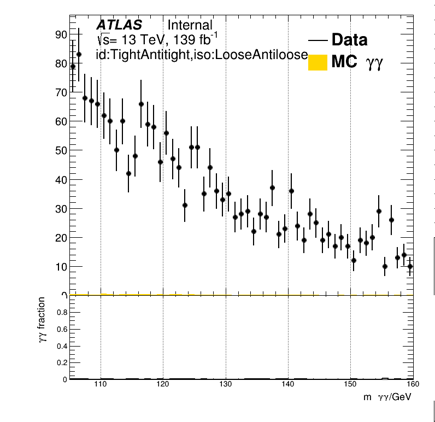
\includegraphics[width= 0.30\textwidth]{figure/bkgtmpls/LT/CR/b4.png} }
  \subfloat[LT category OO bin5]{ 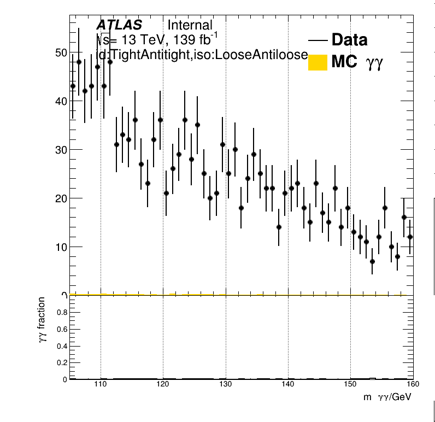
\includegraphics[width= 0.30\textwidth]{figure/bkgtmpls/LT/CR/b5.png} }
  \subfloat[LT category OO bin6]{ 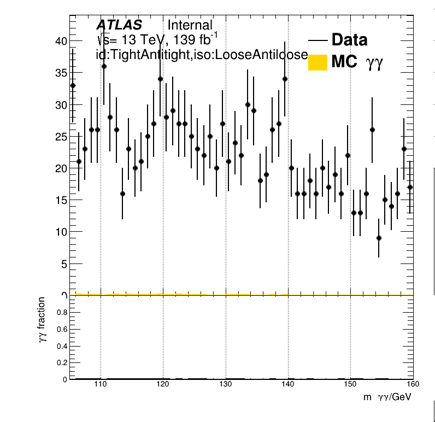
\includegraphics[width= 0.30\textwidth]{figure/bkgtmpls/LT/CR/b6.png} } \\
  \subfloat[LL category OO bin1]{ 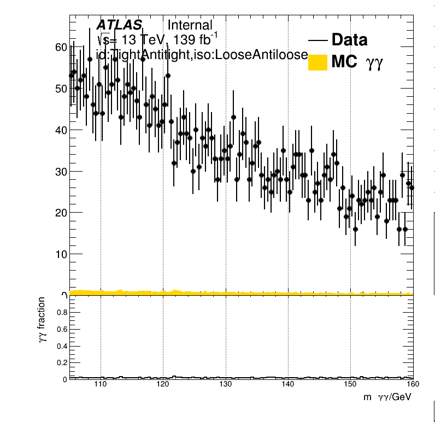
\includegraphics[width= 0.30\textwidth]{figure/bkgtmpls/LL/CR/b1.png} }
  \subfloat[LL category OO bin2]{ 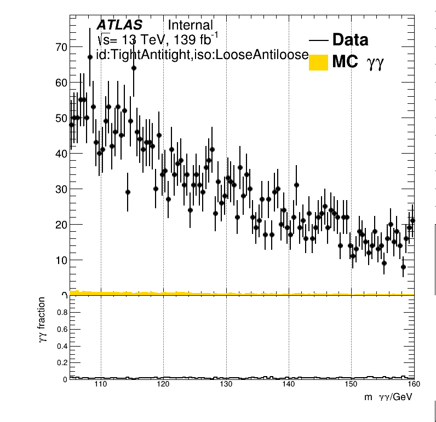
\includegraphics[width= 0.30\textwidth]{figure/bkgtmpls/LL/CR/b2.png} }
  \subfloat[LL category OO bin3]{ 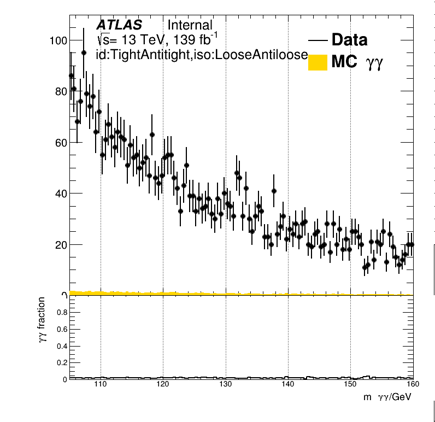
\includegraphics[width= 0.30\textwidth]{figure/bkgtmpls/LL/CR/b3.png} } \\
  \subfloat[LL category OO bin4]{ 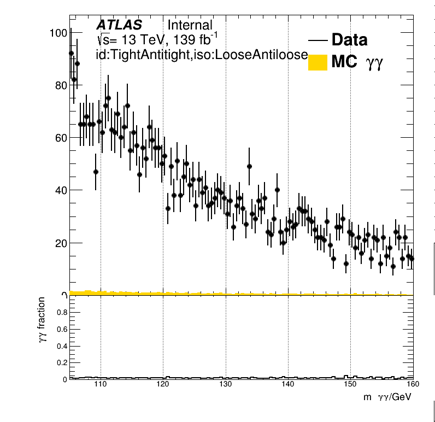
\includegraphics[width= 0.30\textwidth]{figure/bkgtmpls/LL/CR/b4.png} }
  \subfloat[LL category OO bin5]{ 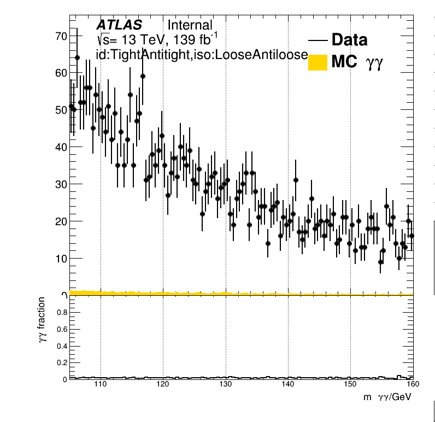
\includegraphics[width= 0.30\textwidth]{figure/bkgtmpls/LL/CR/b5.png} }
  \subfloat[LL category OO bin6]{ 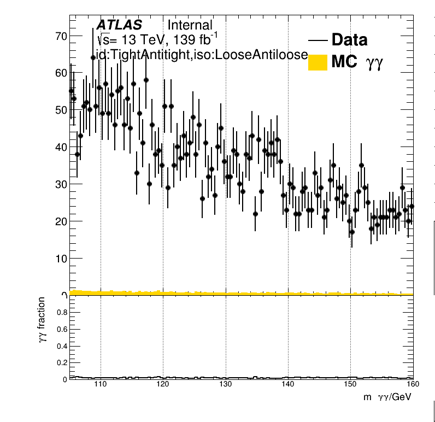
\includegraphics[width= 0.30\textwidth]{figure/bkgtmpls/LL/CR/b6.png} } \\
  \caption{Control region data in all categories and OO bins.}
  \label{fig:yjCR}
\end{figure}
\clearpage

\begin{figure}[htbp]
  \centering
  \subfloat[TT category OO bin1]{ 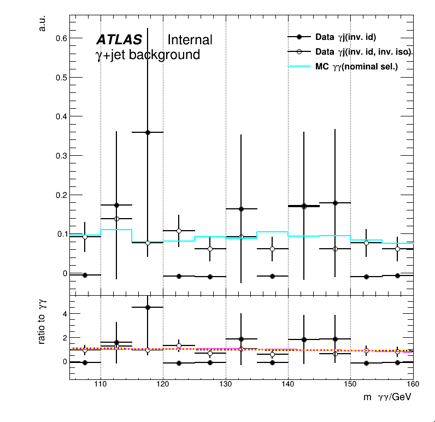
\includegraphics[width= 0.30\textwidth]{figure/bkgtmpls/TT/reweight/b1.png} }
  \subfloat[TT category OO bin2]{ 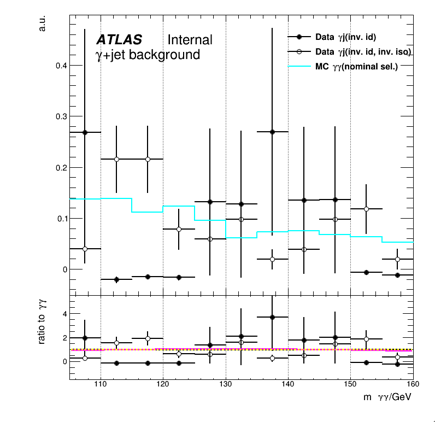
\includegraphics[width= 0.30\textwidth]{figure/bkgtmpls/TT/reweight/b2.png} }
  \subfloat[TT category OO bin3]{ 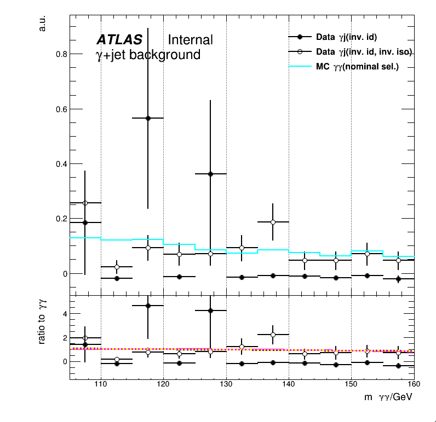
\includegraphics[width= 0.30\textwidth]{figure/bkgtmpls/TT/reweight/b3.png} } \\
  \subfloat[TT category OO bin4]{ 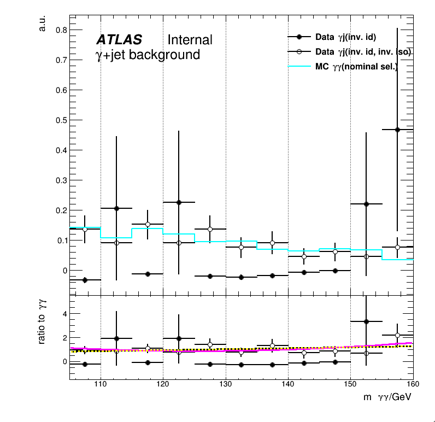
\includegraphics[width= 0.30\textwidth]{figure/bkgtmpls/TT/reweight/b4.png} }
  \subfloat[TT category OO bin5]{ 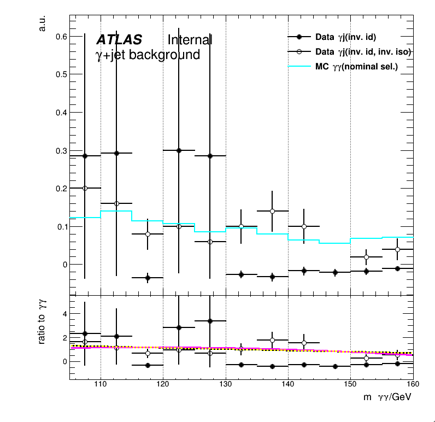
\includegraphics[width= 0.30\textwidth]{figure/bkgtmpls/TT/reweight/b5.png} }
  \subfloat[TT category OO bin6]{ 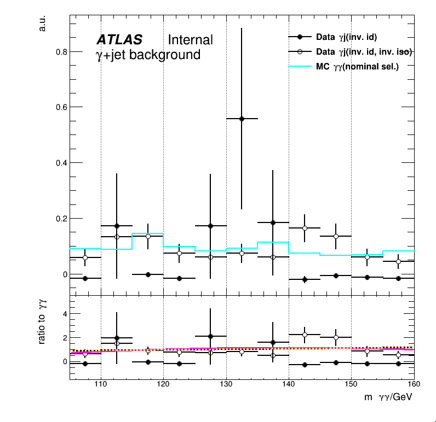
\includegraphics[width= 0.30\textwidth]{figure/bkgtmpls/TT/reweight/b6.png} } \\
  \subfloat[TL category OO bin1]{ 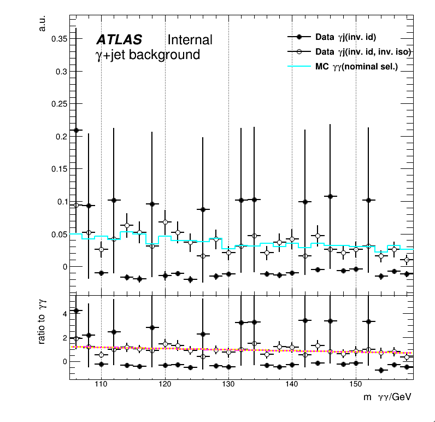
\includegraphics[width= 0.30\textwidth]{figure/bkgtmpls/TL/reweight/b1.png} }
  \subfloat[TL category OO bin2]{ 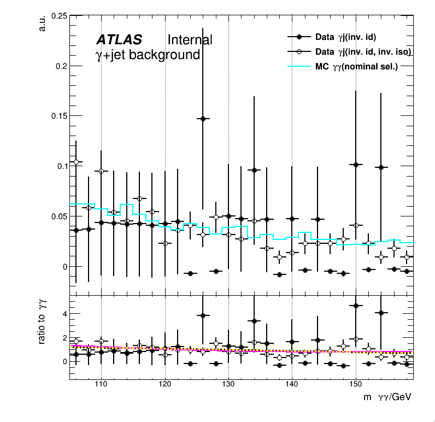
\includegraphics[width= 0.30\textwidth]{figure/bkgtmpls/TL/reweight/b2.png} }
  \subfloat[TL category OO bin3]{ 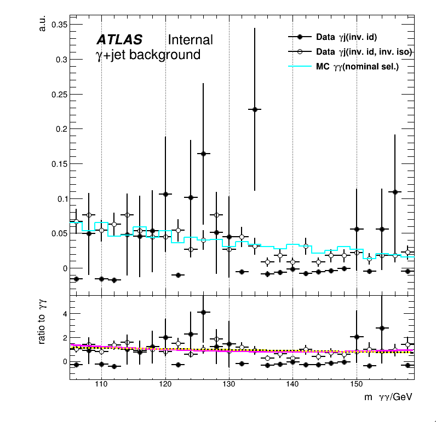
\includegraphics[width= 0.30\textwidth]{figure/bkgtmpls/TL/reweight/b3.png} } \\
  \subfloat[TL category OO bin4]{ 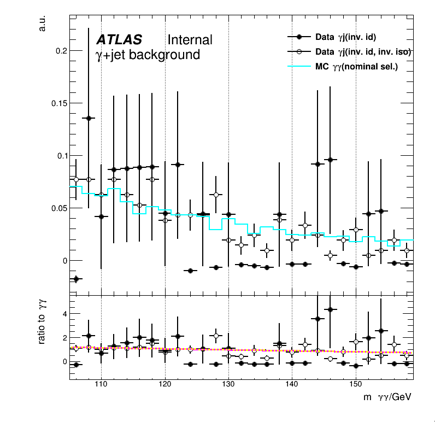
\includegraphics[width= 0.30\textwidth]{figure/bkgtmpls/TL/reweight/b4.png} }
  \subfloat[TL category OO bin5]{ 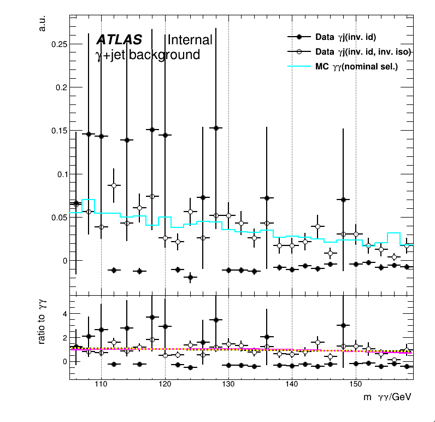
\includegraphics[width= 0.30\textwidth]{figure/bkgtmpls/TL/reweight/b5.png} }
  \subfloat[TL category OO bin6]{ 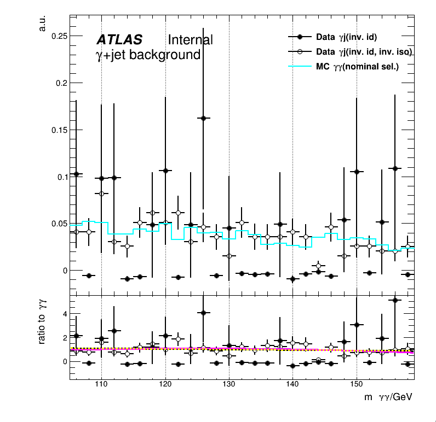
\includegraphics[width= 0.30\textwidth]{figure/bkgtmpls/TL/reweight/b6.png} } \\
\end{figure}
\clearpage
\begin{figure}[htbp]
\centering
  \subfloat[LT category OO bin1]{ 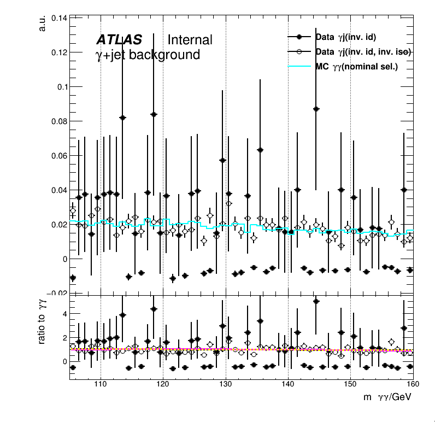
\includegraphics[width= 0.30\textwidth]{figure/bkgtmpls/LT/reweight/b1.png} }
  \subfloat[LT category OO bin2]{ 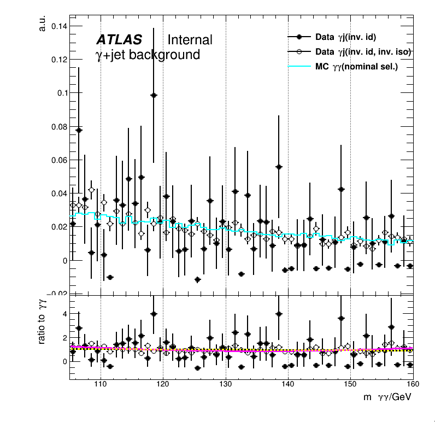
\includegraphics[width= 0.30\textwidth]{figure/bkgtmpls/LT/reweight/b2.png} }
  \subfloat[LT category OO bin3]{ 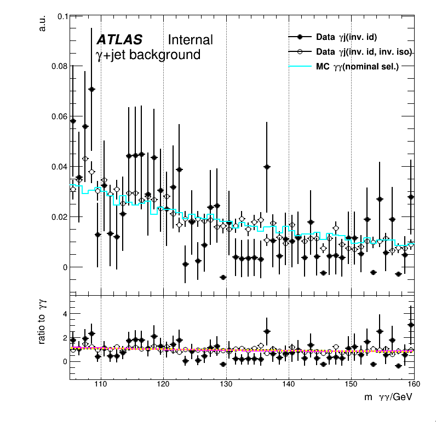
\includegraphics[width= 0.30\textwidth]{figure/bkgtmpls/LT/reweight/b3.png} } \\
  \subfloat[LT category OO bin4]{ 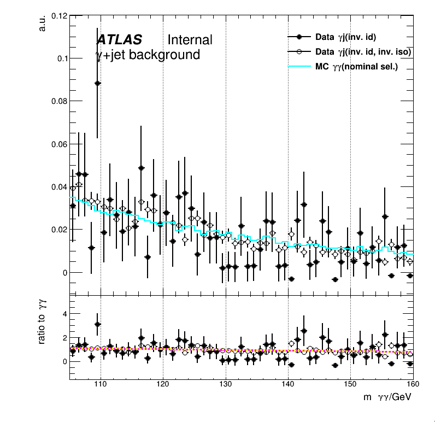
\includegraphics[width= 0.30\textwidth]{figure/bkgtmpls/LT/reweight/b4.png} }
  \subfloat[LT category OO bin5]{ 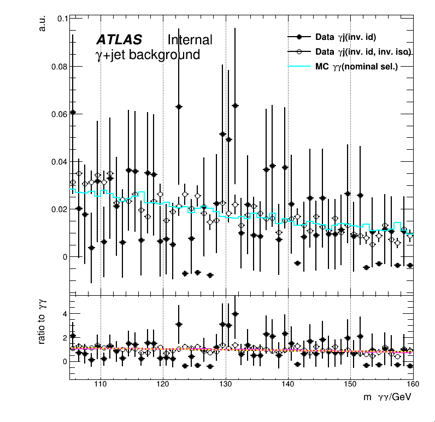
\includegraphics[width= 0.30\textwidth]{figure/bkgtmpls/LT/reweight/b5.png} }
  \subfloat[LT category OO bin6]{ 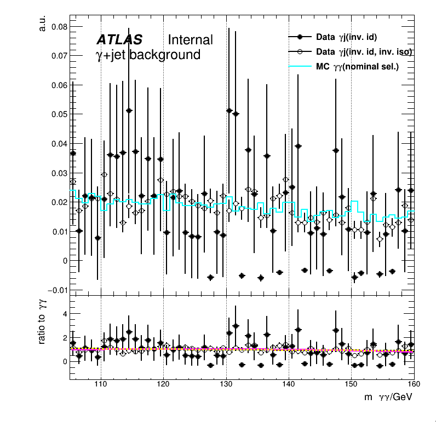
\includegraphics[width= 0.30\textwidth]{figure/bkgtmpls/LT/reweight/b6.png} } \\
  \subfloat[LL category OO bin1]{ 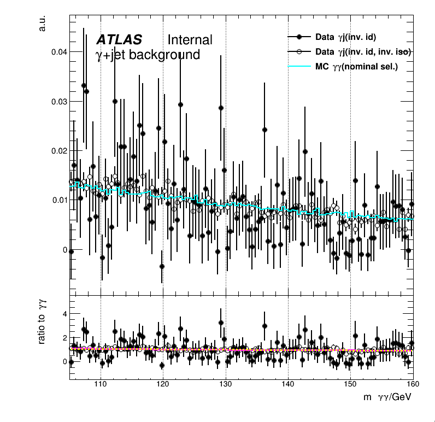
\includegraphics[width= 0.30\textwidth]{figure/bkgtmpls/LL/reweight/b1.png} }
  \subfloat[LL category OO bin2]{ 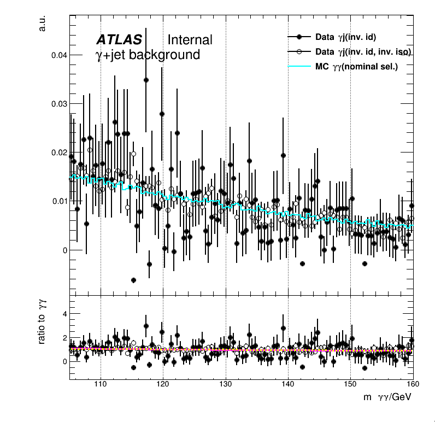
\includegraphics[width= 0.30\textwidth]{figure/bkgtmpls/LL/reweight/b2.png} }
  \subfloat[LL category OO bin3]{ 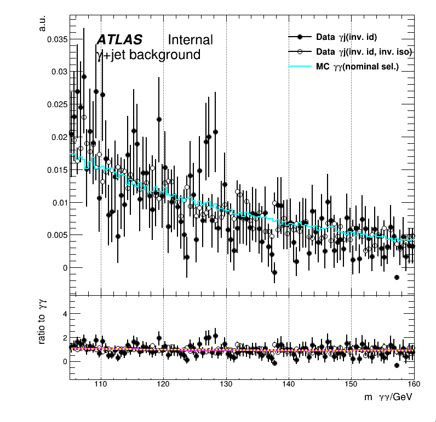
\includegraphics[width= 0.30\textwidth]{figure/bkgtmpls/LL/reweight/b3.png} } \\
  \subfloat[LL category OO bin4]{ 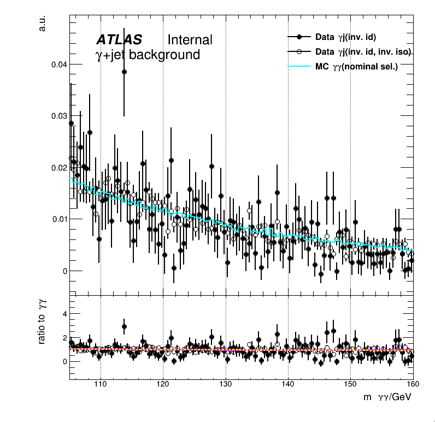
\includegraphics[width= 0.30\textwidth]{figure/bkgtmpls/LL/reweight/b4.png} }
  \subfloat[LL category OO bin5]{ \includegraphics[width= 0.30\textwidth]{figure/bkgtmpls/LL/reweight/b5.png} }
  \subfloat[LL category OO bin6]{ \includegraphics[width= 0.30\textwidth]{figure/bkgtmpls/LL/reweight/b6.png} } \\
  \caption{Reweight \yy MC with a linear function to match the \yjet+\jetjet shape in each bins and categories.}
  \label{fig:yyReweight}
\end{figure}
\clearpage

\begin{figure}[htbp]
  \centering
  \subfloat[TT category OO bin1]{ \includegraphics[width= 0.30\textwidth]{figure/bkgtmpls/TT/raw_tmpl/b1.png} }
  \subfloat[TT category OO bin2]{ \includegraphics[width= 0.30\textwidth]{figure/bkgtmpls/TT/raw_tmpl/b2.png} }
  \subfloat[TT category OO bin3]{ \includegraphics[width= 0.30\textwidth]{figure/bkgtmpls/TT/raw_tmpl/b3.png} } \\
  \subfloat[TT category OO bin4]{ \includegraphics[width= 0.30\textwidth]{figure/bkgtmpls/TT/raw_tmpl/b4.png} }
  \subfloat[TT category OO bin5]{ \includegraphics[width= 0.30\textwidth]{figure/bkgtmpls/TT/raw_tmpl/b5.png} }
  \subfloat[TT category OO bin6]{ \includegraphics[width= 0.30\textwidth]{figure/bkgtmpls/TT/raw_tmpl/b6.png} } \\
  \subfloat[TL category OO bin1]{ \includegraphics[width= 0.30\textwidth]{figure/bkgtmpls/TL/raw_tmpl/b1.png} }
  \subfloat[TL category OO bin2]{ \includegraphics[width= 0.30\textwidth]{figure/bkgtmpls/TL/raw_tmpl/b2.png} }
  \subfloat[TL category OO bin3]{ \includegraphics[width= 0.30\textwidth]{figure/bkgtmpls/TL/raw_tmpl/b3.png} } \\
  \subfloat[TL category OO bin4]{ \includegraphics[width= 0.30\textwidth]{figure/bkgtmpls/TL/raw_tmpl/b4.png} }
  \subfloat[TL category OO bin5]{ \includegraphics[width= 0.30\textwidth]{figure/bkgtmpls/TL/raw_tmpl/b5.png} }
  \subfloat[TL category OO bin6]{ \includegraphics[width= 0.30\textwidth]{figure/bkgtmpls/TL/raw_tmpl/b6.png} } \\
\end{figure}
\clearpage
\begin{figure}[htbp]
\centering
  \subfloat[LT category OO bin1]{ \includegraphics[width= 0.30\textwidth]{figure/bkgtmpls/LT/raw_tmpl/b1.png} }
  \subfloat[LT category OO bin2]{ \includegraphics[width= 0.30\textwidth]{figure/bkgtmpls/LT/raw_tmpl/b2.png} }
  \subfloat[LT category OO bin3]{ \includegraphics[width= 0.30\textwidth]{figure/bkgtmpls/LT/raw_tmpl/b3.png} } \\
  \subfloat[LT category OO bin4]{ \includegraphics[width= 0.30\textwidth]{figure/bkgtmpls/LT/raw_tmpl/b4.png} }
  \subfloat[LT category OO bin5]{ \includegraphics[width= 0.30\textwidth]{figure/bkgtmpls/LT/raw_tmpl/b5.png} }
  \subfloat[LT category OO bin6]{ \includegraphics[width= 0.30\textwidth]{figure/bkgtmpls/LT/raw_tmpl/b6.png} } \\
  \subfloat[LL category OO bin1]{ \includegraphics[width= 0.30\textwidth]{figure/bkgtmpls/LL/raw_tmpl/b1.png} }
  \subfloat[LL category OO bin2]{ \includegraphics[width= 0.30\textwidth]{figure/bkgtmpls/LL/raw_tmpl/b2.png} }
  \subfloat[LL category OO bin3]{ \includegraphics[width= 0.30\textwidth]{figure/bkgtmpls/LL/raw_tmpl/b3.png} } \\
  \subfloat[LL category OO bin4]{ \includegraphics[width= 0.30\textwidth]{figure/bkgtmpls/LL/raw_tmpl/b4.png} }
  \subfloat[LL category OO bin5]{ \includegraphics[width= 0.30\textwidth]{figure/bkgtmpls/LL/raw_tmpl/b5.png} }
  \subfloat[LL category OO bin6]{ \includegraphics[width= 0.30\textwidth]{figure/bkgtmpls/LL/raw_tmpl/b6.png} } \\
  \caption{Final background templates.}
  \label{fig:BkgData-MC}
\end{figure}
\clearpage


\subsubsection{Background smoothing}
\label{ssec:bkg_smoothing}
\textcolor{red}{Need Simplification} \\

Because of the limited statistics of the simulation samples used in the calculation, the value
of the spurious signal systematic uncertainty is subject to significant statistical fluctuations within
many of the analysis categories~\cite{Hyneman:2712576}. Statistical fluctuations in the background-only sample may cause
signal-like bumps, which are then fit as signal by the spurious signal procedure. These statistical fluctuations do
not capture the shape mismodeling from the analytic function, and they often drastically inflate the
value of the systematic.

Although simply producing additional simulation samples would alleviate the issue of statistical
fluctuations fitted as spurious signal, producing more simulated events is computationally
expensive. Additionally, producing events which fall into specific phase spaces is often highly inefficient. 
Therefore, an alternative solution using the available simulation samples is preferred. 

A Gaussian Process (GP) is defined as a set of random processes, where all finite subsets of these
processes have a multivariate normal distribution~\cite{ebden2015gaussian}. 
Given a finite dataset – such as the bin contents of a smooth histogram – with corresponding
mean and covariance matrices, a Gaussian Process may be defined. The “correct” mean and the
covariance, however, are not necessarily well defined, as they encode specific assumptions about
the underlying dataset. In practice, the two quantities are fit to a finite dataset using a minimization
algorithm. In the case of a one-dimensional histogram with a finite number of bins, the mean can
be interpreted as a “rough” description of the underlying shape. The diagonal elements of the
covariance matrix represent the error of each bin while the off-diagonal elements specify
how “similar” the bin content of two different bins should be.

The covariance matrix can be simplified through the introduction of a kernel, which analytically
determines the level of correlation between two distinct points (i.e., the length scales in X at which points are expected to influence one another in Y). Two useful kernels are the Radial Basis Function (RBF) kernel and the Gibbs kernel~\cite{3569,Gibbs}. 

The RBF kernel has one hyperparameter, the constant length scale $l$, and it is defined as

\begin{equation}
K_\text{RBF}(x,x') = exp\left(\frac{-(x-x')^2}{2l^2}\right)
\end{equation}

The RBF kernel is useful for mostly-flat functions. However, for smoothly-falling functions, it is likely that nearby points will be more correlated in some regions than in others, so a constant length scale is a suboptimal model. The Gibbs kernel allows the length scale $l(x)$ to vary linearly as a function of $x$, and thus has two hyperparameters: the initial length scale and the length scale slope. The Gibbs kernel function is: 

\begin{equation}
K_\text{Gibbs}(x, x') = \frac{\sqrt{2l(x)l(x')}}{l(x)^2 + l(x')^2 } \cdot exp\left( \frac{-(x-x')^2}{l(x)^2 + l(x')^2} \right)
\end{equation}


The background templates used in the spurious signal test for the analysis categories are all smooth,
roughly exponentially falling distributions with statistical fluctuations. Fitting a background template
using Gaussian Process Regression (using the Gibbs kernel with the errors as determined by the initial templates) 
offers a consistent method of estimating the underlying smooth shape of the template, without the problematic fluctuations. 
Notably, the GP smoothing technique makes no assumption on the underlying distribution other than that it is smooth and falling, hence the choice of functional form from the spurious signal test will not be biased.

The hyperparameters (initial length scale and length scale slope) are allowed to vary over a range specified by the user; the optimal hyperparameters within this range are determined by the Gaussian Process fitting procedure.

A GP is fit to the original (noisy) background template in each category. The GP mean in the fits is defined as an exponential function,
the parameters of which are obtained by a fit to the original background template. The exponential
shape has been observed to be a sufficiently close guess for the categories used by the analysis.
However, in cases where the input template has very few statistics (less than about ten events per
bin on average), the resulting GP fit may be nearly identical to the mean exponential shape. This
issue occurs when the statistical uncertainties of the original template are so large that the template
is fully compatible with the preliminary exponential shape. Although the exponential shape
is technically an adequate descriptor of the template shape, the choice of the exponential mean
does bias the functional choice of the spurious signal test in this case. Therefore, a check has been
added to re-perform the GP fit using a flat mean in cases where the resulting GP shape and the
mean exponential shape disagree with a $\chi^2/DoF < 0.1$.

The resulting smoothed shape obtained from the GP fit is then saved as a new histogram. This
smoothed histogram is passed as the background template to the spurious signal test, which then
determines the background functional form and spurious signal systematic uncertainty as described
in \Sect{\ref{ssec:spurious_signal}}.

Note that based on previous study, the GPR method can only remain effectively unbiased for smoothly-falling templates containing more than an average of 20 Monte Carlo events/ bin ~\cite{HyyCoupling_140ifb}. 
The TT and TL categories in this analysis even do not have sufficient statistics for GPR. Only LT and LL categories used this method, and the treatment of TT and TL is discussed in Section ~\ref{sssec:bkg_functions}. 

Examples of the smoothed templates are presented in \Fig{\ref{fig:exampleGPR}} for a sample category with a high
level of statistics and for a category with a very low level of statistics.
The original templates are shown as well, for comparison. The data sidebands are also shown for
validation, although the GP smoothing technique does not take into account the data sidebands.

\begin{figure}[htbp]
  \centering
  \subfloat[LT category OO bin1]{ \includegraphics[width= 0.30\textwidth]{figure/bkgtmpls/LT/smooth_tmpl/b1.png} }
  \subfloat[LT category OO bin2]{ \includegraphics[width= 0.30\textwidth]{figure/bkgtmpls/LT/smooth_tmpl/b2.png} }
  \subfloat[LT category OO bin3]{ \includegraphics[width= 0.30\textwidth]{figure/bkgtmpls/LT/smooth_tmpl/b3.png} } \\
  \subfloat[LT category OO bin4]{ \includegraphics[width= 0.30\textwidth]{figure/bkgtmpls/LT/smooth_tmpl/b4.png} }
  \subfloat[LT category OO bin5]{ \includegraphics[width= 0.30\textwidth]{figure/bkgtmpls/LT/smooth_tmpl/b5.png} }
  \subfloat[LT category OO bin6]{ \includegraphics[width= 0.30\textwidth]{figure/bkgtmpls/LT/smooth_tmpl/b6.png} } \\
  \subfloat[LL category OO bin1]{ \includegraphics[width= 0.30\textwidth]{figure/bkgtmpls/LL/smooth_tmpl/b1.png} }
  \subfloat[LL category OO bin2]{ \includegraphics[width= 0.30\textwidth]{figure/bkgtmpls/LL/smooth_tmpl/b2.png} }
  \subfloat[LL category OO bin3]{ \includegraphics[width= 0.30\textwidth]{figure/bkgtmpls/LL/smooth_tmpl/b3.png} } \\
  \subfloat[LL category OO bin4]{ \includegraphics[width= 0.30\textwidth]{figure/bkgtmpls/LL/smooth_tmpl/b4.png} }
  \subfloat[LL category OO bin5]{ \includegraphics[width= 0.30\textwidth]{figure/bkgtmpls/LL/smooth_tmpl/b5.png} }
  \subfloat[LL category OO bin6]{ \includegraphics[width= 0.30\textwidth]{figure/bkgtmpls/LL/smooth_tmpl/b6.png} } \\
  \caption{LT and LL category background templates after GPR smooth.}
  \label{fig:exampleGPR}
\end{figure}


%The smoothed background templates used in this analysis and the spurious signal values extracted from them can be found in the \App{\ref{sec:GPR_templates}}.


%Extensive validation tests were performed with the GP smoothing technique in order to ensure that the smoothing itself does not introduce a substantial bias. These tests primarily use “toy” templates – randomly-generated background templates constructed from either simulated diphoton events or from the probability distribution function of a known analytic function. We find that GPR remains effectively unbiased for smoothly-falling templates containing more than an average of 20 Monte Carlo events/ bin. These procedures to validate the GPR smoothing are reported in \App{\ref{sec:GPR_validation}}.





\subsection{Spurious signal test}
\label{ssec:spurious_signal}

The background \myy shape, for each analysis category, is described using an analytic function whose parameters and normalization are fitted to data. The choices for the analytic function that has been considered are:
\begin{itemize}
\item Exponential Function: $f(\myy) = e^{c\cdot \myy}$
\item Exponential Function of $2^{nd}$ Order Polynomial: $f(\myy) = e^{c_1\cdot m^2_{\gamma\gamma}+c_2\cdot \myy}$
\item Exponential Function of $3^{nd}$ Order Polynomial: $f(\myy) = e^{c_1\cdot m^3_{\gamma\gamma}+c_2\cdot m^2_{\gamma\gamma}+c_3\cdot \myy}$
\item Bernstein polynomial of order $N$: $B_{N}(\myy) = \sum_{i=0}^N c_i\cdot b_{i,N}$ with $b_{i,N} = \begin{pmatrix}N\\i\end{pmatrix}\myy^i (1-\myy)^{N-i}$, N=3, 4, 5
\item First-Order Power Law Function: $f(\myy) = \myy^c$
\end{itemize}
The method to select the functional form in each category is based on the spurious signal. The spurious signal test is described in more detail in \cite{Hasib:2238687}.

To perform the spurious signal test, the full analytic signal plus background model is fitted to a background-only template for each category separately. The fit is performed in the nominal diphoton mass range of $105 \leq \myy \leq \SI{160}{\GeV}$. The number of fitted signal events as a function of the Higgs mass is computed in intervals of \SI{1}{\GeV} within the diphoton mass range of $120 \leq \myy \leq \SI{130}{GeV}$. Negative fluctuations are taken into account. The number of spurious signal events $N_{sp}$ is then defined as the maximum of the absolute value of the fitted number of signal events within the signal diphoton mass sub-range. The statistical error is always taken into account.

The choice of analytic function is done such that the function satisfies at least one of the following criteria:
\begin{itemize}
\item $N_{sp}$ < 10\% $N_{s,exp}$, where $N_{s,exp}$ is the expected number of signal events within the SM in the category ($\mu_{sp} = N_{sp} / N_{s,exp}$)
\item $N_{sp}$ < 20\% $\sigma_{bkg}$, where $\sigma_{bkg}$ is the statistical uncertainty on the fitted number of signal events, when fitting the signal+background model to a background only Asimov dataset ($Z_{sp} = N_{sp} / \sigma_{bkg}$).
\end{itemize}

If multiple functions pass the test, then the one with the least number of parameters is chosen.

%The study including all the categories (also non-ttH) will be performed in the future in accordance with the method described in the previous iteration of the analysis. Due to the higher statistics, new functions (with more parameters) might be needed for the high statistics event categories, as for example the ggH categories. For the ttH only analysis, this does not need to be done.
%These should pass at least the 
%Due to the limitation of MC statistic amount, 
    A relaxed spurious signal criteria, that are made to accommodate $2\sigma$ local statistical fluctuations in the MC template, in case the MC statistics is small compared to the expected signal. This is done by defining a new variable:
\begin{align}
    \zeta_{sp} = 
   \begin{cases}
N_{sp} + 2\Delta_{MC},~~~~ N_{sp} + 2\Delta_{MC}<0\\
N_{sp} - 2\Delta_{MC},~~~~ N_{sp} - 2\Delta_{MC}>0\\
0, ~~~~~~~~~~~~~~~~~~~~~~~\text{otherwise}\\
\end{cases}
 \label{eq:relSpuriousSignalMetric}
\end{align}
where $\Delta_{MC}$ is a local statistical fluctuation of the MC background template. This is illustrated in \Fig{\ref{fig:relaxed_ss_cartoon}}. This newly defined variable should then pass the criteria as $N_{sp}$ before. 

For categories with at least 100 data events in the sideband regions defined as $105 < m_{\gamma\gamma} < 120$ GeV or $130 < m_{\gamma\gamma} < 160$ GeV, the background functions are selected to result in a $|S_{\text{spur}}|$ that is smaller than either 10\% of the total expected Higgs boson signal event ($S_{\text{exp}}$) or 20\% of the statistical uncertainty of the fitted signal yield ($\sigma_{\text{exp}}$). The fit of the analytic function to the background template is required to yield a $\chi^2$ probability of at least $1\%$~\footnote{The $\chi^2$ is computed with a background template uniformly binned over $105<m_{\gamma\gamma}<160$ GeV. The number of bins is 22, and the degrees of freedom used in the computation is 21 - $N_{\text{pars}}$, the number of free function parameters.}.

If multiple functions pass the requirements, the one with the smallest number of degrees of freedom is chosen. If no function passes, the spurious signal requirement is relaxed to  
 $\zeta_{sp}$ < 10\% $N_{s,exp}$ or $\zeta_{sp}$ < 20\% $\sigma_{bkg}$.
For 28 out of the 88 categories, these relaxed conditions were used. 
It's to be emphasized that even the relaxed condition is used, the background uncertainty is still $N_{sp}$ from the nominal approach of spurious signal study.





\subsubsection{Treatment of low-statistic cetegories}
\label{sssec:bkg_functions}

The determination of analytical functions is part of the result of spurious signal study, however, for low stastics categories with a background template suffering of very large statistical flucttuation we introduce a preliminary step. The straight use of the spurious signal procedure on these templates, in fact, would potentially lead to select a function with large number of degrees of freedom to accomodate these statistical fluctuation, and these function can prove to be dangerous when used on data. For this reason, for categories with less then 100 events in the \myy\ sidebads, we restrict the selection of the modeling function to exponential of first, second and third order, collectively described by:
\begin{equation}
  f_i{x} = e^{\sum_{i=0}^2 a_i x^i}
\end{equation}
where $x = \myy$. 

We accept as modeling function the $f_i$ function with the lowest number of degrees of freedom for which the addition of more degrees of freedom does not lead to a significant improvement in the quality of the fit of the \myy\ sidebands. 
To this purpose, we checked the likelihood ratio between the fits to the side-band data with two different background models:
\begin{equation}
\lambda_{(1,2)} = -2ln(L_{1}/L_{2})
\end{equation}
Where $L_{1}$ and $L_{2}$ are the likelihood values of the two fits.

The distributions of these test statistics are computed with \myy\
 side-band data, fitting it with two models and calculating the value of the test statistics.  
 Once the distributions of the test-statistics
are computed, we can reject the simpler (less parameters) background
model by checking the P-value $P(\lambda >= \lambda_{\mathrm{data}})$ with the $\lambda$ measured in data ($\lambda_{\mathrm{data}}$).
This procedure to reject simpler background function is called Wald test.

Figure ~\ref{fig:Wtest} shows plots of the Wald-test on the low-statistic categories. All of the categories selected exponential function as the final decison.
Where the lowest P-value among all categories are around 3$\%$, corresponding to a significance of 2.2 $\sigma$ standard deviations.  
The background uncertainty for these categories will be the spurious signal from exponential function.

As a cross-check, a F-test is also performed in Appendix ~\ref{append:ss}, and we draw the same conclusion that all of the categories can select exponential function.
The reason we use Wald test to decide the background function is the fits on side-band data are un-bin fit (so that it's consistent with the final result), 
    there might be bias if we calculate the $\chi^2$ values in an artifical bin-size for the F-test. In this case the Wald test based on likelihood ratio is more reliable.

\begin{figure}[htbp]
  \centering
  \subfloat[TT category OO bin1]{ \includegraphics[width= 0.30\textwidth]{figure/bkgtmpls/TT/wald/b1.png} }
  \subfloat[TT category OO bin2]{ \includegraphics[width= 0.30\textwidth]{figure/bkgtmpls/TT/wald/b2.png} }
  \subfloat[TT category OO bin3]{ \includegraphics[width= 0.30\textwidth]{figure/bkgtmpls/TT/wald/b3.png} } \\
  \subfloat[TT category OO bin4]{ \includegraphics[width= 0.30\textwidth]{figure/bkgtmpls/TT/wald/b4.png} }
  \subfloat[TT category OO bin5]{ \includegraphics[width= 0.30\textwidth]{figure/bkgtmpls/TT/wald/b5.png} }
  \subfloat[TT category OO bin6]{ \includegraphics[width= 0.30\textwidth]{figure/bkgtmpls/TT/wald/b6.png} } \\
  \subfloat[TL category OO bin1]{ \includegraphics[width= 0.30\textwidth]{figure/bkgtmpls/TL/wald/b1.png} }
  \subfloat[TL category OO bin2]{ \includegraphics[width= 0.30\textwidth]{figure/bkgtmpls/TL/wald/b2.png} }
  \subfloat[TL category OO bin3]{ \includegraphics[width= 0.30\textwidth]{figure/bkgtmpls/TL/wald/b3.png} } \\
  \subfloat[TL category OO bin4]{ \includegraphics[width= 0.30\textwidth]{figure/bkgtmpls/TL/wald/b4.png} }
  \subfloat[TL category OO bin5]{ \includegraphics[width= 0.30\textwidth]{figure/bkgtmpls/TL/wald/b5.png} }
  \subfloat[TL category OO bin6]{ \includegraphics[width= 0.30\textwidth]{figure/bkgtmpls/TL/wald/b6.png} } \\
  \caption{Wald test in TT and TL categories. In all OO bins the first order exponential function shows the lower p value and is selected.}
  \label{fig:Wtest}
\end{figure}




\subsection{Background modelling results}
\label{ssec:bck_results}

The determined analytical functions modeling the baground in each category entering the measureument are found in Table~\ref{tab:spurious_sig} , as well as the corresponsing Spurious Signal bias.
The background only fit on the background templates based on MC samples is shown in Figure ~\ref{fig:bkgonly}


\begin{table}[htbp]
\centering
\small
\begin{tabular}{l|l|l|l|l|l|l|l|l}
\hline
           & \multicolumn{2}{c|}{TT} & \multicolumn{2}{c|}{TL} & \multicolumn{2}{c|}{LT} & \multicolumn{2}{c|}{LL} \\ \hline
           & Selected func. & maxS   & Selected func. & maxS   & Selected func. & maxS   & Selected func. & maxS   \\ \hline \hline
bin0       & Exp            & -0.29  & Exp            & -0.468 & Exp            & 0.87   & Exp            & 0.885  \\ \hline
bin1       & Exp            & 0.582  & Exp            & -0.882 & Exp            & -0.534 & Exp            & 1.54   \\ \hline
bin2       & Exp            & 0.235  & Exp            & -0.355 & Pow            & 0.437  & ExpPoly2       & -1.64  \\ \hline
bin3       & Exp            & 0.409  & Exp            & -0.304 & Pow            & 0.642  & Exp            & -0.718 \\ \hline
bin4       & Exp            & -0.404 & Exp            & 0.779  & Exp            & 0.775  & Exp            & -1.19  \\ \hline
bin5       & Exp            & 0.293  & Exp            & 0.408  & Exp            & 0.627  & Exp            & 0.52   \\ \hline
\end{tabular}
\caption{The final background modelling decision and the size of spurious signal uncertainties.}
\label{tab:spurious_sig}
\end{table}


\begin{figure}[htbp]
  \centering
  \subfloat[TT category OO bin1]{ \includegraphics[width= 0.30\textwidth]{figure/bkgfit/TT/b1.pdf} }
  \subfloat[TT category OO bin2]{ \includegraphics[width= 0.30\textwidth]{figure/bkgfit/TT/b2.pdf} }
  \subfloat[TT category OO bin3]{ \includegraphics[width= 0.30\textwidth]{figure/bkgfit/TT/b3.pdf} } \\
  \subfloat[TT category OO bin4]{ \includegraphics[width= 0.30\textwidth]{figure/bkgfit/TT/b4.pdf} }
  \subfloat[TT category OO bin5]{ \includegraphics[width= 0.30\textwidth]{figure/bkgfit/TT/b5.pdf} }
  \subfloat[TT category OO bin6]{ \includegraphics[width= 0.30\textwidth]{figure/bkgfit/TT/b6.pdf} } \\
  \subfloat[TL category OO bin1]{ \includegraphics[width= 0.30\textwidth]{figure/bkgfit/TL/b1.pdf} }
  \subfloat[TL category OO bin2]{ \includegraphics[width= 0.30\textwidth]{figure/bkgfit/TL/b2.pdf} }
  \subfloat[TL category OO bin3]{ \includegraphics[width= 0.30\textwidth]{figure/bkgfit/TL/b3.pdf} } \\
  \subfloat[TL category OO bin4]{ \includegraphics[width= 0.30\textwidth]{figure/bkgfit/TL/b4.pdf} }
  \subfloat[TL category OO bin5]{ \includegraphics[width= 0.30\textwidth]{figure/bkgfit/TL/b5.pdf} }
  \subfloat[TL category OO bin6]{ \includegraphics[width= 0.30\textwidth]{figure/bkgfit/TL/b6.pdf} } \\
\end{figure}
\clearpage
\begin{figure}[htbp]
\centering
  \subfloat[LT category OO bin1]{ \includegraphics[width= 0.30\textwidth]{figure/bkgfit/LT/b1.pdf} }
  \subfloat[LT category OO bin2]{ \includegraphics[width= 0.30\textwidth]{figure/bkgfit/LT/b2.pdf} }
  \subfloat[LT category OO bin3]{ \includegraphics[width= 0.30\textwidth]{figure/bkgfit/LT/b3.pdf} } \\
  \subfloat[LT category OO bin4]{ \includegraphics[width= 0.30\textwidth]{figure/bkgfit/LT/b4.pdf} }
  \subfloat[LT category OO bin5]{ \includegraphics[width= 0.30\textwidth]{figure/bkgfit/LT/b5.pdf} }
  \subfloat[LT category OO bin6]{ \includegraphics[width= 0.30\textwidth]{figure/bkgfit/LT/b6.pdf} } \\
  \subfloat[LL category OO bin1]{ \includegraphics[width= 0.30\textwidth]{figure/bkgfit/LL/b1.pdf} }
  \subfloat[LL category OO bin2]{ \includegraphics[width= 0.30\textwidth]{figure/bkgfit/LL/b2.pdf} }
  \subfloat[LL category OO bin3]{ \includegraphics[width= 0.30\textwidth]{figure/bkgfit/LL/b3.pdf} } \\
  \subfloat[LL category OO bin4]{ \includegraphics[width= 0.30\textwidth]{figure/bkgfit/LL/b4.pdf} }
  \subfloat[LL category OO bin5]{ \includegraphics[width= 0.30\textwidth]{figure/bkgfit/LL/b5.pdf} }
  \subfloat[LL category OO bin6]{ \includegraphics[width= 0.30\textwidth]{figure/bkgfit/LL/b6.pdf} } \\
  \caption{Background only fit on the background templates based on MC samples. }
  \label{fig:bkgonly}
\end{figure}


